\documentclass[10pt,a4paper]{article}
\usepackage[margin=2.2cm]{geometry}
\usepackage{fontspec}
\usepackage{kotex}
\setmainfont{Apple SD Gothic Neo}
\setsansfont{Apple SD Gothic Neo}
\usepackage{amsmath,amssymb}
\usepackage{graphicx}
\usepackage{booktabs}
\usepackage{caption}
\usepackage[dvipsnames]{xcolor}
\usepackage[colorlinks=true,linkcolor=MidnightBlue,citecolor=MidnightBlue,
            urlcolor=MidnightBlue]{hyperref}
\usepackage{titlesec}
\titleformat{\section}{\large\bfseries}{\thesection}{0.6em}{}
\titleformat{\subsection}{\normalsize\bfseries}{\thesubsection}{0.5em}{}
\captionsetup{font=small,labelfont=bf}
\setlength{\parskip}{0.35em}
\setlength{\parindent}{0pt}

\usepackage{mdframed}
\newmdenv[linewidth=0.4pt,linecolor=gray!60,backgroundcolor=gray!5,
          innertopmargin=6pt,innerbottommargin=6pt,skipabove=8pt,skipbelow=8pt]{claimbox}
\newcommand{\claim}[2]{\begin{claimbox}\textbf{주장.} #1\par\smallskip
  \textcolor{gray!70}{\textbf{반증 조건.} #2}\end{claimbox}}

\title{\bfseries 다섯 번, 검사가 먼저 틀렸다\\[2pt]
\large 회귀 시험이 감사를 감사한다}
\author{월드모델 실험실 · 노트 669 · 671 · 672 · 676 · 677}
\date{2026-08-06}
\begin{document}\maketitle

\section{한 줄}

이 세션에서 감사 검사를 넷 새로 세웠다. 그 넷이 실제 결함 다섯을 잡았다. 그런데
\textbf{그 넷 자체에도 구멍이 다섯 개 있었고, 다섯 번 다 ``통과''라는 결과가 아니라
회귀 시험이나 결과를 눈으로 본 것이 드러냈다.}

\section{왜 검사를 새로 세웠나}

노트 546 · 549 가 \emph{``장부와 코드가 따로 자란다''}를 두 번 적었다. 노트 670 이 세
번째를 찾았는데 모양이 달랐다 --- \textbf{고침 자체가 장부에만 있었다.} 대장 노트 650 에
\emph{``갈래 합집합 결함을 고쳤다''}고 적혀 있는데 \verb|git log --all -p| 에
\verb|cumsum| 이 \textbf{0회}였고, 뒤따른 두 노트(650 · 651)가 결함 있는 축을 쟀다.

주석으로 적은 금지는 다음 사람이 안 읽는다(노트 598). 그래서 넷을 세웠다.

\begin{center}
\begin{tabular}{lll}
\toprule
검사 & 무엇을 보나 & 이 세션에서 잡은 것 \\
\midrule
\verb|law_only_leak| (656) & 법칙 전용 자료가 축에 새었나 & --- \\
\verb|claimed_fixes| (670) & 대장이 주장하는 고침이 코드에 있나 & 유령 고침 1 \\
\verb|t_propagation| (668·671) & \texttt{T} 를 안 넘기는 자리 & \verb|g_alive| 1 \\
\verb|dead_numbers| (672·677) & 정정된 숫자가 살아 있는 문서에 남았나 & 3 \\
\bottomrule
\end{tabular}
\end{center}

\claim{\textbf{감사는 자료만 재면 안 되고 저장소와 기록 자신도 재야 한다.} 앞의 다섯
검사(덮음 · 출처 · 절단 · 신선도 · 대조)는 \emph{자료}를 재고, 새 넷은 \emph{우리}를
잰다. 되돌아간 고침 · 안 넘긴 인자 · 낡은 숫자는 자료 문제가 아니라 기록 문제이고,
\textbf{그것이 두 노트를 헛돌게 했다.}}
{새 넷이 오랫동안 0건만 내면 유지 비용이 값보다 크다. 지금은 세션 하나에서 5건을
잡았으므로 그 판정을 뒤로 미룬다.}

\section{그런데 그 검사들이 다섯 번 먼저 틀렸다}

\begin{figure}[t]\centering
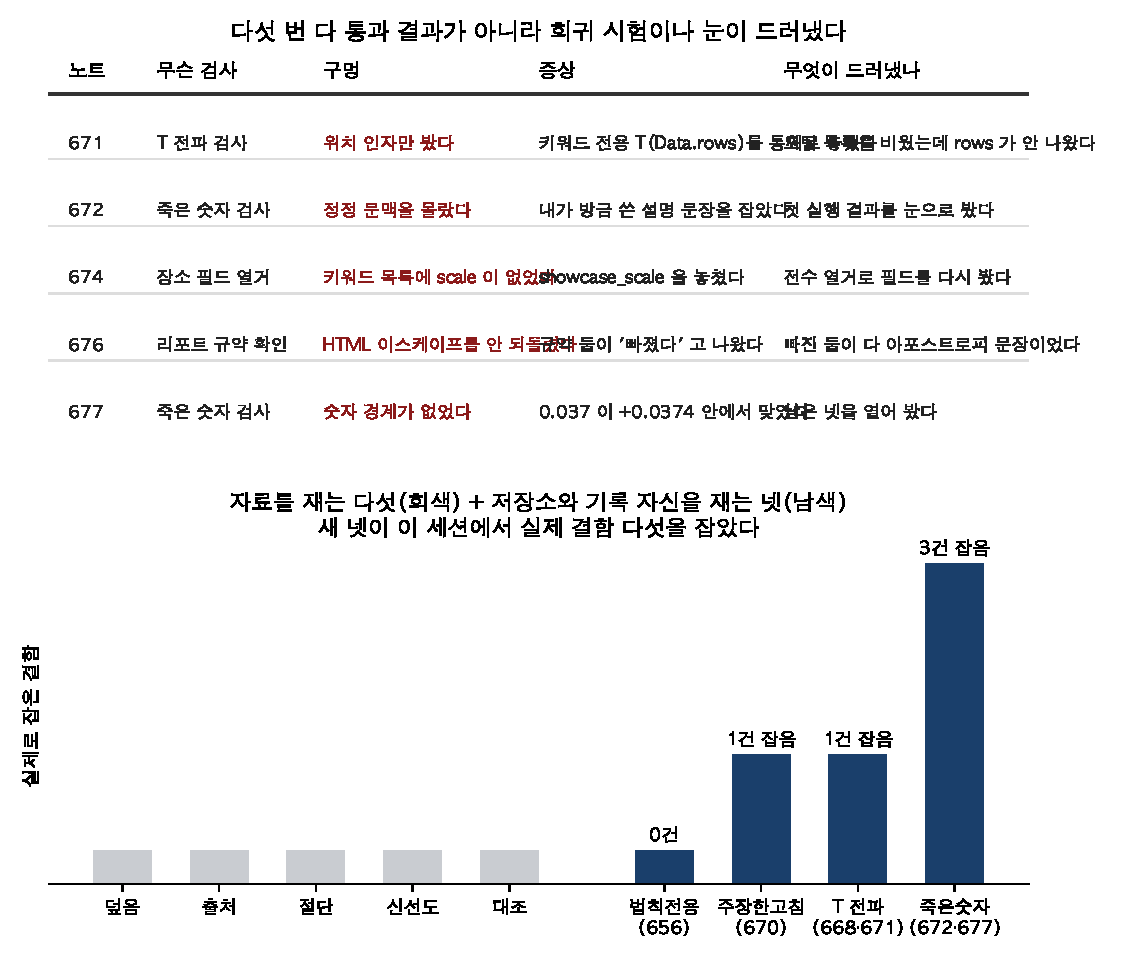
\includegraphics[width=0.99\textwidth]{figs/fivetimes.pdf}
\caption{위: 다섯 사례. \textbf{구멍}은 검사가 못 본 것이고 \textbf{증상}은 그래서
나온 잘못된 결과다. 오른쪽 칸이 핵심이다 --- \textbf{무엇이 드러냈나.} 아래: 자료를
재는 다섯과 저장소를 재는 넷.}
\end{figure}

특히 두 사례가 서로 거울이다.

\textbf{노트 674}(장소 필드 열거)는 키워드 목록으로 훑어 ``장소 필드 0개''를 얻었다.
전수 열거로 보니 \verb|showcase_scale| 이 있었고 그 안에 \emph{``서울 구로구
고척스카이돔''}이 들어 있었다. \textbf{내 키워드 목록에 `scale' 이 없었다.}

\textbf{노트 677}은 반대다. \verb|dead_numbers| 에 \verb|0.037| 을 넣자 네 곳이
걸렸는데 열어 보니 전부 \verb|+0.0374|(노트 551 이웃 효과) · \verb|+0.0373|
(\verb|goods_scale|)이었다. \textbf{더 긴 숫자의 앞부분}으로 맞은 것이다. 그리고 그
결함은 노트 674 가 \verb|hood_sgg| 에서 진단한 것과 \textbf{같은 기제}다 --- 멤버
이름 `미아'를 강북구 미아동으로 읽은 것(31건 중 6건 = 19\%).

\claim{\textbf{문자열로 찾는 검사는 경계를 정해야 한다} --- 숫자 경계 · 단어 경계 ·
HTML 태그 · 이스케이프. 이 세션에서 그 넷이 각각 한 번씩 걸렸다. 그리고
\textbf{조항을 코드로 옮겼는데 그 코드가 조항을 어겼다} --- 노트 674 가 진단한
부분 문자열 결함이 이틀 뒤 내가 세운 감사 안에 있었다.}
{한글 단어 경계는 아직 안 걸었다(지금 표에 한글 값이 없어서다). 그러므로 이 주장의
``넷''은 완전한 목록이 아니고 \textbf{다음에 한글 값을 넣을 때 다섯째가 나온다}.}

\section{그래서 규약이 하나 생겼다}

\begin{center}
\textbf{검사를 세울 때 회귀 시험을 같이 세운다.}\\
\textbf{그리고 문자열로 찾는 검사는 경계를 정한다.}
\end{center}

\textbf{왜 회귀 시험이 필요한가.} 다섯 번 다 ``통과''는 아무것도 안 말했다. 노트 671
에서는 오탐 목록을 비웠는데 \verb|rows| 가 안 나오는 것을 보고 알았고, 노트 672 에서는
첫 실행이 \emph{내가 방금 쓴 설명 문장}을 잡는 것을 보고 알았고, 노트 677 에서는 남은
넷을 열어 보고 알았다. \textbf{검사가 무엇을 잡는지는 통과가 아니라 실패를 심어야
보인다.}

\section{그리고 무해한 누출도 하나 있었다}

노트 669 는 결이 다르다. 사전학습(\verb|state/fieldmodel|)의 \textbf{표본 구성}이
새고 있었다 --- 어느 동네가 판에 드는지를 \emph{전 구간} 덮음으로 골랐다. 노트 645 는
\emph{값}(정규화 통계)이 새는 것을 막았는데 이것은 \textbf{표본 구성}이 새는 것이라
층이 다르다.

고쳐서 재니 \textbf{동네 261 $\to$ 261, 차이 0건}이고 검증 R$^2$ 가
$0.1098 \to 0.1098$ 로 \emph{정확히} 같았다. \textbf{누출은 구조적으로 실재했지만 이
자료에서는 비어 있다.} 예측이 맞았고 기제도 맞았다 --- 시군구 자료가 2020-01 부터
전국에 고르게 쌓여 있어서다.

\claim{\textbf{학습 구간으로만 정해야 하는 것은 값이 아니라 결정이다.} 정규화 통계 ·
\textbf{어느 행이 판에 드나} · 어느 열을 쓰나 · 어느 지평을 고르나 --- 넷이 다 같은
병이다. 이번 것이 무해했다는 이유로 고침을 되돌리지 않는다(자료가 자라면 깨진다).}
{새 시군구가 생기거나 수집이 중간에 끊기면 이 무해함이 사라진다 --- 그것이 고침을
남기는 이유다.}

\subsection*{덤 --- 기록된 숫자 둘이 낡아 있었다}

같은 측정에서 사전학습 검증 R$^2$ 가 대장에 \textbf{$+0.1639$}(위약 $-0.0206$)로
적혀 있는데 지금 재면 $0.1098$(위약 $-0.0074$)이다. 원인 둘 --- \textbf{방문자 자료가
자랐고}(지금 2{,}349일) \textbf{위약 설계가 기록에 없었다.} 후자가 더 나쁘다: 숫자만
있고 설계가 없으면 재현이 안 되고 고침 전후를 견줄 수도 없다. 그래서 위약을 정의해
적었다(목표를 동네 안에서 시간축으로 섞음).

\textbf{자료가 자라는 원천 위에서 잰 숫자는 재현 조건(자료 스냅샷)을 같이 적는다.}

\end{document}
